\chapter{Game Tree Search}
\label{c:game-tree-search}
In many games with relatively simple rules but deep strategy complexity, computer programs have surpassed the best human players by considerable margin. In most cases, the successful technique has been the same: building a search tree of the possible decisions, and evaluating the resulting game states with a domain-specific evaluation function - often accompanied by efficient alpha-beta pruning. Probably the most notable field for these successes are chess programs, like \textit{Deep Blue} which won a widely publicized exhibition match against then chess world champion Garry Kasparov in 1997. Since then, other programs like Fritz and Shredder achieved constant performances on par with or above the best human players, adding chess to the growing list of games dominated by computer programs (similar examples including Checkers and Othello are mentioned in \cite{Billings2006}).  

The approach has not been successful for the game of \textit{Go}, however, owing to the high branching factor and vast search space, and the fact that goals and sub-goals are very difficult to assess with heuristic evaluation.

This chapter will outline the strategies to solve game decision problems with search trees, and the required adaptations to use these algorithms in a non-deterministic and imperfect information game like poker.

\section{Deterministic games with perfect information}
\label{sec:perfectinformation}
Considering games with two players, \cite{Russell2003} explains the generic game tree search for deterministic, turn-taking, two-player, zero-sum games of perfect information. Although poker doesn't fulfill most of these attributes - cards are not dealt deterministic, ring-games can involve more than two-players and there is obviously no perfect information - the basic strategies outlined here can still be applied to find a solution on what action to take in a poker game - as shown in later chapters.

The basic game problem for this algorithm involves two player, called \texttt{MAX} and \texttt{MIN}, named after their strategic targets (\texttt{MAX} has to maximize payoffs, \texttt{MIN} tries to minimize them). \texttt{MAX} moves first, and then both player take alternating turns until the game is over. At the end of the game, the winning player gained something while the loosing player is punished (whatever the incentives are to win, respectively not to loose). A game can be formally defined as a search problem with these components (according to \cite{Russell2003}):

\begin{itemize}
	\item The \textbf{initial state}, which includes the board position and identifies the player to move.
	\item A \textbf{successor function}, which returns a list of \textit{(move, state)} pairs, each indicating a legal move and the resulting state.
	\item A \textbf{terminal test}, which determines when the game is over. States where the game has ended are called terminal states.
	\item A \textbf{utility function} (also called an objective function or payoff function), which gives a numeric value for the terminal states. In chess, the outcome is a win, loss, or draw, with values +1, -1, or 0. Some games have a wider variety of possible outcomes; the payoffs in backgammon range from +192 to -192. The payoffs in poker depend on the exact betting sequences leading to a terminal state.
\end{itemize}

In game theory, this representation is called the extensive form representation, opposed to the normal-form it allows easy analysis thanks to its tree-graph visualization of the game (\cite{Gilpin2007}).
 
Starting with the initial state as a node, with legal moves as links to resulting states (until a terminal state is reached), figure \ref{fig:tictactoe-tree1} shows part of a game tree for tic-tac-toe. From the initial state, \texttt{MAX} has nine possible moves. After those, the game alternates between \texttt{MAX} placing \texttt{X}s and \texttt{MIN} placing \texttt{O}s until a leaf node corresponding to a terminal state, where all fields are filled of one player has marked three fields in a row, is reached. The number on each leaf node indicates the utility value of the terminal state from the point of view of \texttt{MAX}; high values are assumed to be good for \texttt{MAX} and bad for \texttt{MIN}. The game tree is represented so that the best move for \texttt{MAX} has to be determined, as he is acting on the initial node.

\begin{figure}[!ht]
\centering
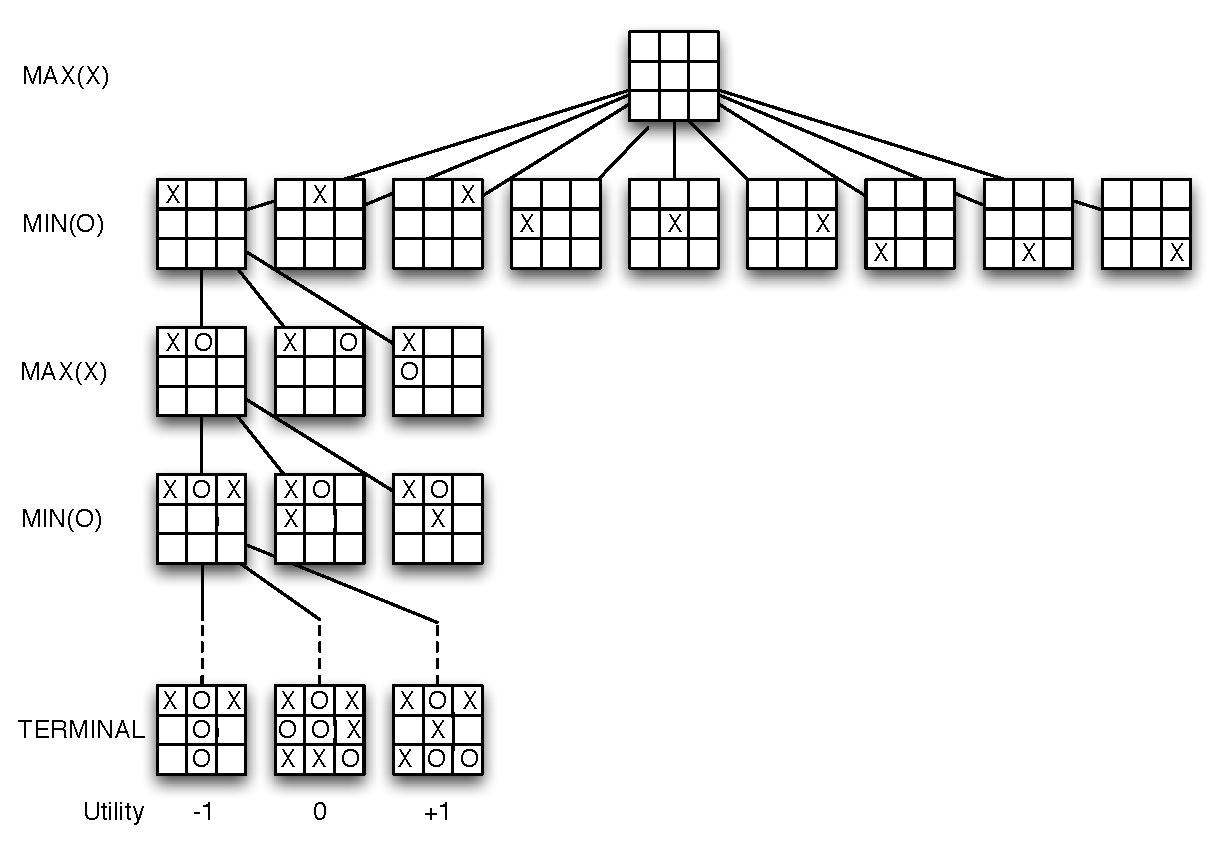
\includegraphics[width=\linewidth]{section03-gametree/figures/tictactoe-tree}
\caption{A partial search tree for the game of tic-tac-toe.}
\label{fig:tictactoe-tree1}
\end{figure}

\subsection{The Minimax Algorithm}
In a normal graph searching problem, the optimal solution would be a sequence of moves leading to a goal state with a high payoff (e.g. a win). In a game though, as \cite{Russell2003} explains, \texttt{MIN} obviously has the power to influence this sequence of moves. \texttt{MAX} must find a contingent strategy, which specifies a first move in the initial state, as well as the following moves in all states resulting from every possible response by \texttt{MIN} to those moves, until all such sequences end in a terminal node. As even tic-tac-toe is too complex to draw the entire game tree (not to speak of limit, or even no-limit poker), a much simpler game is presented in figure \ref{fig:trivialgame-tree}. Here, \texttt{MAX} is given three moves at the root node, labeled $a_1$, $a_2$ and $a_3$ to choose from. The possible replies by \texttt{MIN} are $b_1$, $b_2$ and $b_3$ if \texttt{MAX} chose $a_1$, $c_1$, $c_2$ and $c_3$ if \texttt{MAX} chose $a_2$ and the nodes designated with $d_n$ if \texttt{MAX} chose $a_3$. This game ends after one move by each player, resulting in a tree that is one move deep, consisting of two half-moves called \textit{ply}s. The payoffs vary in a range between 2 to 14.

\begin{figure}[!ht]
\centering
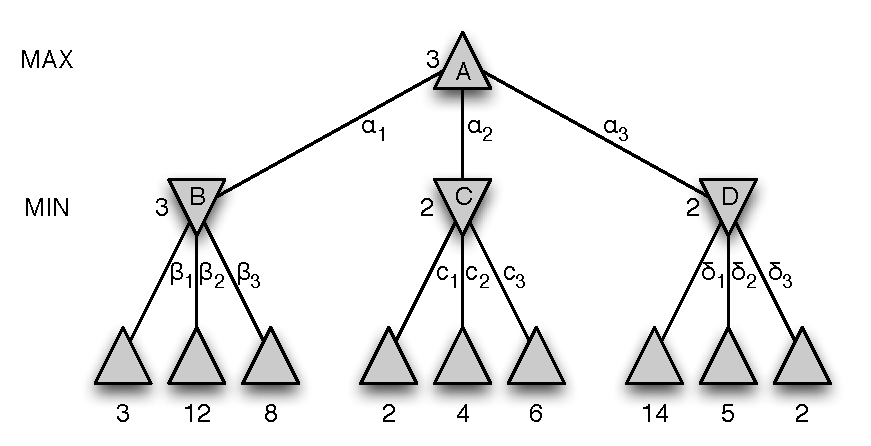
\includegraphics[width=\linewidth]{section03-gametree/figures/trivialgame-tree}
\caption{Game tree of the trivial game from \cite{Russell2003}. The $\bigtriangleup$ nodes are decision nodes of \texttt{MAX}, the $\bigtriangledown$ for \texttt{MIN}. The terminal nodes show the utility values for \texttt{MAX}.}
\label{fig:trivialgame-tree}
\end{figure}

After this game tree for the problem at hand has been created, the optimal strategy can be determined by examining the payoff of each non-terminal node, called the \textbf{minimax value}. Based on the premise that both player play optimal, the minimax value of a node is the utility (for \texttt{MAX}) of being in the corresponding state. Given a choice, \texttt{MAX} will prefer to move to a state of maximum value, whereas \texttt{MIN} prefers a state of minimum value. \cite{Russell2003} forms the following formula \ref{eq:minimax}: 

\begin{equation}
Minimax-Value(n) = 
 \left\{ \begin{array}{lll}
Utility(n) 															& \mbox{if n is a terminal state} \\
max_{s\in Successors(n)} Minimax-Value(s) & \mbox{if n is a MAX node} \\
min_{s\in Successors(n)} Minimax-Value(s) & \mbox{if n is a MIN node}
\end{array}
\right.
\label{eq:minimax}
\end{equation}

In figure \ref{fig:trivialgame-tree} the nodes are already marked with their minimax values. At the first \texttt{MIN} node, labeled $B$, \texttt{MIN} can choose between sucessors with values 3,12,8. As \texttt{MIN} tries to minimize the utility, $B$ gets the minimax value of 3. Analogue, the other two \texttt{MIN} nodes have a minimax value of 2. As the root node is a \texttt{MAX} node, the solution to this game problem will be the decision leading to the node with the highest minimax value: action $a_1$ with a expected payoff of 3. As \cite{Russell2003} mentions, this result assumes that \texttt{MIN} also plays optimally. This assumption only makes sense in deterministic games with perfect information. In this case, there may be other strategies against suboptimal opponents that do better than the minimax strategy; but these strategies necessarily do worse against optimal opponents. More about that will be outlined in section {sec:optimalvsmaximal} about situation where deviation from an optimal strategy is advantgeous or necessarily.

The minimax-algorithm uses a simple recursive computation, proceeding all the way down to the leaves, and then backing up the minimax values as the recursion unwinds. In figure \ref{fig:trivialgame-tree}, the algorithm first recurses down to the three bottomleft nodes, and uses the utility function on them to discover that their values are 3, 12, and
8 respectively. Then it takes the minimum of these values, 3, and returns it as the backed-up value of node B. A similar process gives the backed up values of 2 for C and 2 for D. Finally, we take the maximum of 3,2, and 2 to get the backed-up value of 3 for the root node. 

The minimax algorithm performs a complete depth-first exploration of the game tree. Unfortunately, for real games (and realtime calculations), the time cost for completely exploring the tree is often impractical. Nevertheless, this alogrithm serves as the basis for the mathematical analysis of games and for more practical, modified algorithms. These include the widly used alpha-beta pruning, adding a evaluation function instead of backing up the utility value or the modifications explained in the  following sections.

\section{Stochastic Games with imperfect information}
\label{c:imperfectinformation} 

Unlike Tic-Tac-Toe or the simplistic game used in figure \ref{fig:trivialgame-tree} many games (e.g. backgammon, monopoly etc.) include some element of random chance. The traditional game tree representation can be extended to include additional chance nodes which represent stochastic events and outcomes. Chance nodes spawn branches for each random outcome, with the same weight for each node (assuming the game uses a fair dice). 
From a search perspective, all of these branches must be considered, and combined to obtain an overall expected value (EV), so the size of the game tree grows multiplicatively with each subsequent chance node. As chance nodes don't maximize or minimize, the alpha beta pruning used in minimax-search is not directly applicable to this class of problems. But similar search algorithms such as *-Minimax \cite{Hauk2006} and Expectiminimax \cite[p. 175-180]{Russell2003} are able to handle this form of uncertainty adequately.

According to  \cite{Billings2006}, the property of stochasticity has not been a major	handicap for computer performance in practical games of chance, like backgammon. For backgammon, a game with perfect information, but a certain factor of chance (the roll of the dice) - artificial intelligence research has lead to excellent evaluation functions learned automatically from self-play (see \cite{Tesauro2002}), resulting in several programs that are at least on par with the best human players, without requiring deep search (see \cite{Hauk2006}) of the whole game tree.

But one major distinguishing factor between poker and other games which are subject to artificial intelligence research is the property of imperfect information. At first sight, it might seem that games of imperfect information are just like games with a probabilistic factor: the cards are dealt randomly and determine the moves available to each player, but all the dice are rolled at the beginning. In reality though, we can't just "roll" all possibly start-hands, calculate our actions and then average somehow. \cite{Russell2003} calls that "averaging over clairvoyance", and it can't be used to solve decision problems. The problem with this naive algorithm is that it assumes that in each possible deal, play will proceed as if all the cards are visible. In reality when information is missing, one must consider what information one will have at each point in the game. The following paragraphs outlines the algorithms currently used in computer poker and which are later applied in the implementation (chapter \ref{chap:implementation}). Other approaches to build a poker agent were summarized in section \ref{s:relatedwork}.

\subsection{Miximax Search}

Like perfect information games, games of imperfect information can be represented graphically as a tree. Nodes represent various states in the game, and edges connecting the nodes represent possible actions which cause a transition from one state/node to another. In an imperfect games, nodes have to be categorized into who is is choosing the action at that game state. In perfect information games, that isn't the case, as the optimal action (and its value) each player chooses can be perfectly deduced. Additionally, like in all games of chance, there are chance nodes, where a random process deals cards, and terminal nodes. 

\begin{figure}[!ht]
\centering
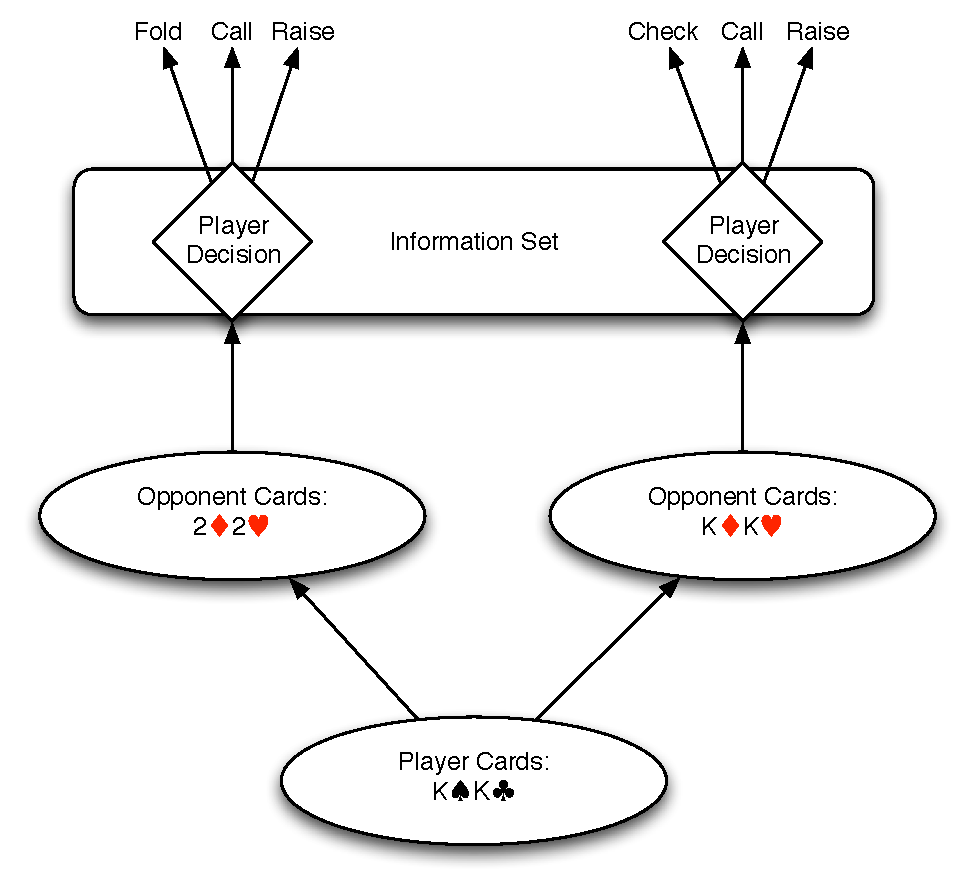
\includegraphics[width=\linewidth]{section03-gametree/figures/information-sets}
\caption{An example of a information set from \cite{Johanson2007}. For the player observing the opponent, its not possible to distinguish the two chance nodes that assign cards to the opponent. An information set contains these game stats that cannot be distinguished.}
\label{fig:information-sets}
\end{figure}

The presence of hidden information means, that the different action nodes of the opponent become indistinguishable, and the player is required to act the same way in all of them. A player can't calculate one action for when the opponent holds a pair, and another for the decision node where he does not hold one. He must find a solution which works in both situations. In game theory, all these action nodes belong to the same information set.  An information set is a set that, for a particular player, establishes all the possible moves that could have taken place in the game so far, given what that player has observed. This means that in Texas Hold'em, all of a player's action nodes that share both the same public information (i.e. the betting actions and community cards) and the same private information (i.e. the player's hole cards) but differ solely because of the opponent's private hidden information (i.e. the opponent's hole cards) belong to the same information set. In the extensive form representation of the game, an information set appears as an oval grouping together a set of player action nodes. (\cite{Schauenberg2006} )

To adapt the game-three for imperfect information games, \textit{information sets} are used. An information set is a set of decision nodes in the game tree that cannot be distinguished from the perspective of an observing player. Since the opponent's cards are hidden in poker, this corresponds to the complete set of all possible opponent holdings in a given situation. 

Obviously, the same strategy (such as a particular mixed strategy) must be applied identically to all of the nodes in the information set, as its obviously impossible to distinguish these states and adapt to them\cite{Billings2006}. 

As an consequence, nodes of the the same imperfect information tree are not independent \cite{Billings2006}.  Thus, a divide-and-conquer search algorithm, such
as the alpha-beta minimax technique explained in \cite{Russell2003}, is not applicable to this class of problems, since sub-trees (of the same information set) cannot be handled independently.

Figure \ref{fig:information-sets} shows an example of information sets. The two choice nodes of the player only vary by the opponents hole cards, and an information set contains these game states.  The player cannot tell if the if the opponent has the pair of twos or the pair of kings. During a game, only the information set the player is in is known - but not the particular game state within that information set.  Since we cannot tell the difference between the game states within the information set, any decision on how to act from that information set must be used for all game states within this set. In Figure \ref{fig:information-sets}, the player cannot decide to raise when the opponent has the pair of twos and call when he has the pair of kings. Since we cannot tell which state we are in, we must choose an action (or probability distribution over actions) to use when we encounter the information set - independent of the possible specific decision node. \cite{Johanson2007}

If the game has perfect information, every information set contains only one member, namely the point actually reached at that stage of the game, the use of information sets doesn't facilitate anything in this case.

\cite{Davidson2002} developed a new method of game-tree search to explore more robust expected value calculations compared, to previous, simulation-based approaches. Instead of using a heuristic evaluation function, it performs a full search to the lead nodes of the imperfect information game tree. At the leaf node, possible card holdings of the opponent are estimated based on the path to the leaf. The expected payouts of the leaf nodes are propagated back to the decision point, and weighted by the estimated probability of each branch.Like minimax in perfect information games, \textit{Miximax} (and it's expansion \textit{Miximix}) choses optimal action for the maximizing (solving the the decision problem) player (or \texttt{MAX} player). But instead of minimizing for the opponent (or \texttt{MIN} player), miximax calculates a weighted sum of all its actions, with weights taken from a estimated probability distribution over the actions (or put differently: an opponent model).

Other than the simulation method (see section \ref{section:simulationbased}), which chooses possible cards first and then generates the actions, Miximax generates the actions, and then estimates the unknown cards at the leaf nodes. This resembles much more the actual viewpoint of a poker player in a poker game. The players act in turn, and only until the end does a showdown reveal the cards of the opponent - if at all. The large majority of hidden-information is placed at the leaves of the search. \cite{Davidson2002} assumes that the action information is more robust than the card information. 


\subsection{Miximax and Miximix}
\label{sec:miximix}
With this expansion of Expectimax to poker, by handling all of the opponent decision nodes within a particular information set as a single node,  \textit{Miximax} and \textit{Miximix} are suitable algorithms for computer poker. As outlined above, they compute the expected value at a opponent decision node by modeling them as chance nodes with probabilities based on the information known or estimated about the domain and the specific opponent.
The backed up EV calculation is used to decide which action the player should performa: bet/raise, check/call, or fold. Given the EV for each of the three (in no-limit poker much more) possible actions, the player (or the algorithm) could simply select the option with the maximum value. In that case, the tree would contain mixed nodes for the opponent's decisions and max nodes for the players decision. This approach is followed with the \textit{Miximax} Algorithm (\textit{Mix-} for the opponents strategy, \textit{-max} for the players strategy).

Always taking the maximum EV could lead to predictable play though. To prevent exploitation by an alert opponent, the algorithm could be modified to use a mixed strategy himself. Although the randomized strategy is transparent to the player, it can be viewed as both actors having mixed nodes, therefore this algorithm is called \textit{Miximix} (\textit{Miximax} therefor being a special case of \textit{Miximix} with player decision nodes having a distribution over only one - optimal - action). 

The implementation of expectimax for action-selection in \cite{Schauenberg2006} uses a Miximix variant which dynamically creates a probability distribution by taking a "Boltzmann soft max" distribution \cite{Sutton1998} over the available actions. This creates a distribution that is biased towards higher-valued actions, but does not completely rule out choosing lower-valued actions. Although \cite{Schauenberg2006} doesn't mention this, \cite{Davidson2002} knows that it obviously makes little sense to choose actions with a negative expected value. This probability distribution is then used to both select actions at the decision node and also to backup expected values there so that the backward induction process can continue up the tree. 

As \cite{Schauenberg2006} stresses, the construction of such a distribution is an open research question regarding the tradeoff between exploration and exploitation (the purer the strategy, the higher the potential reward as well as the risk of getting exploited in the long run). The more biased the distribution is toward higher valued actions (with the extreme in \textit{Maximix}), the more the player bases his actions on its current beliefs about the opponent. This implies that it is less likely to explore taking other actions which it currently believes to be worse just to try and discover if better alternatives exist. Intuitively, addressing the exploration/exploitation tradeoff gives a player the means to take a short-term loss to achieve a long-term gain.

\cite{Schauenberg2006} sees his usage of Gibbs or Boltzmann distributions \cite{Sutton1998} simplistic. For my thesis, I have decided to even use \textit{Maximix}, as the emphasis should lie on the opponent model, and this adapts stronger. Calculating distinct distributions for each player decision node also adds a non-trivial cost of computation, which is already pretty high with the rather rich opponent model explained in the later chapters.

\subsection{Calculation example}

Figure \ref{fig:miximax} shows a situation, where the deciding player (\texttt{MAX}) is on the river and has to choose the next action. We assume a rather strong hand. For simplicity, the example is for limit-poker (so the player doesn't have to choose a betting amount). The model shows, that if the player checks, the opponent will also check 20\% of the time and bet 80\% of the time. If the player bets, the opponent will fold 20\%, call 60\% and raise 20\% of the time. The expected action frequencies are noted on the square nodes which represent the opponent actions. The players node are circular. The leaves are hexagons, marked with the estimated payoff (counted from the original decision point, already including costs to reach this point).

\begin{figure}[!ht]
\centering
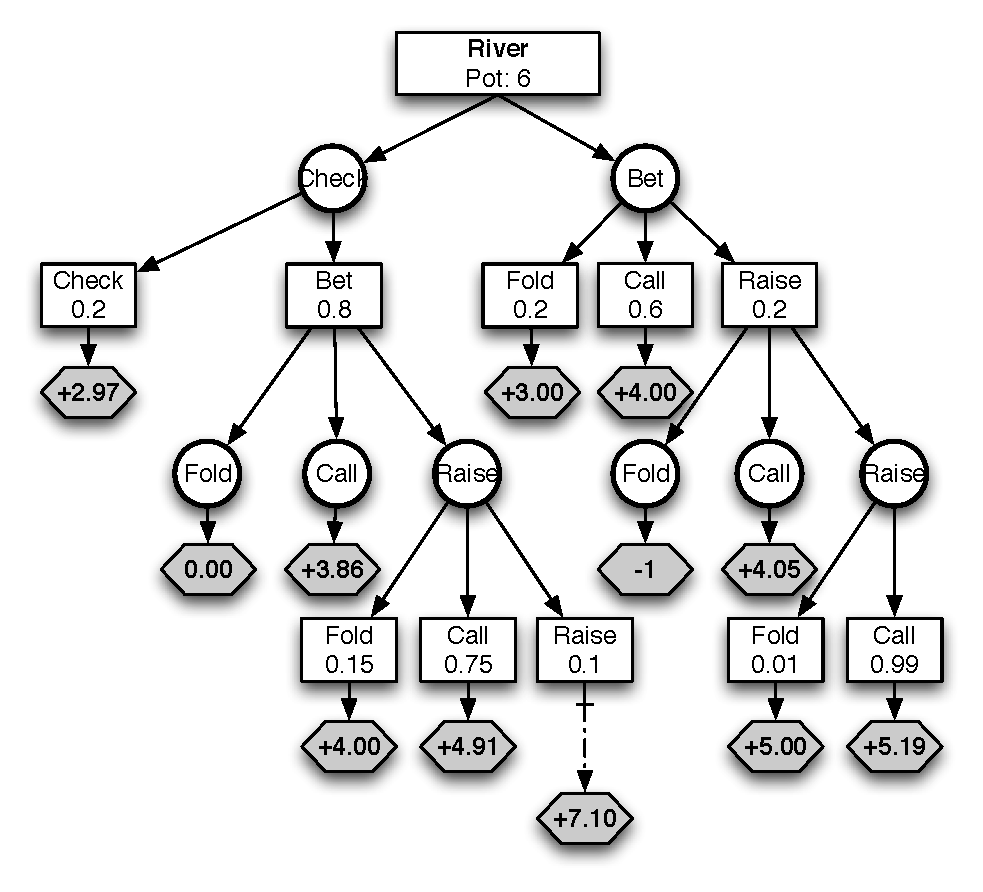
\includegraphics[width=\linewidth]{section03-gametree/figures/miximax}
\caption{A game tree with opponent modeling and hand evaluation for a river decision (example values taken from \cite{Davidson2002})}
\label{fig:miximax}
\end{figure}

Since the player is given a (very) strong hand, all leafs representing showdowns have a positive EV. In betting sequences where the opponent raises, the estimate is less optimistic, since the opponent is more likely to have a stronger hand. Backing up the values at the leaves, gives the estimates of the expected value shown in figure \ref{fig:miximax2}. We can compute, that the EV of checking is equal to 0.2 times the EV of the subtree where the player and the opponent checks, and 0.8 times the EV where the player checks and the opponent bets. In this given example, the player would proceed to Check, since the EV of checking is 4.59, higher than the 4.04 of betting.

\begin{figure}[!ht]
\centering
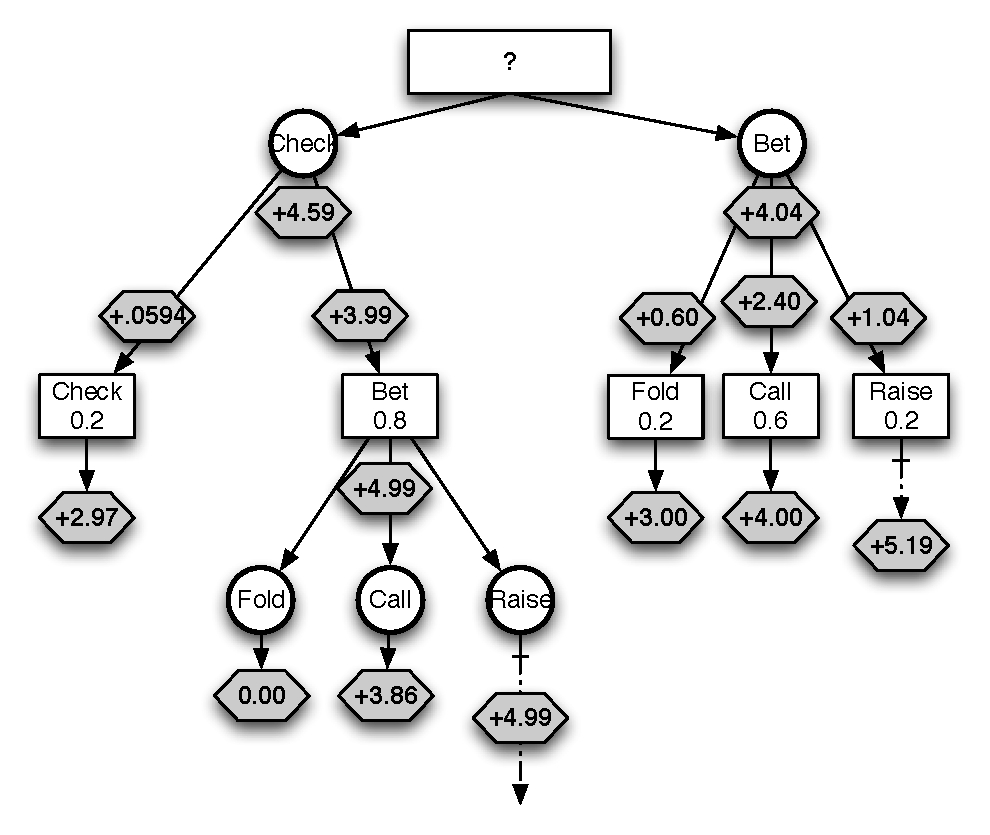
\includegraphics[width=\linewidth]{section03-gametree/figures/miximax2}
\caption{Example of the EV calculation for checking and betting for the decision in figure \ref{fig:miximax}}
\label{fig:miximax2}
\end{figure}

To repeat the calculations used in Miximax-Search (out of \cite{Davidson2002}, \cite{Schauenberg2006} and \cite{Billings2006b}): 

\begin{itemize}
	\item To calculate the expected value for one of the \textbf{players decisions}, the weighted sum of its children's values is used. The weights are the probability of the occurrence of a certain response from the opponent. Let $Pr(A_i)$ be the estimated probability that the opponent will respond with child move $i$ to the decision node $A$, and let $n$ be the number of legal options of the opponent. The EV of the player's action $A$ becomes:
\begin{equation}
	EV(A) = \sum_{i=1}^n Pr(A_i)\times EV(A_i)
\end{equation}
	\item To calculate the expected value for one of the \textbf{opponents decisions} we take the maximum EV of the children (the players responses). Here, the maximum is chosen for simplicity, to employ a mixed strategy, this can be modified to a more accurate function. Such strategies are mentioned in the next section \ref{sec:miximix}
	\begin{equation}
	EV(B)=max(EV(B_{fold}),EV(B_{call}),EV(B_{raise}))
	\end{equation}
Or in general, for n choices (like in no-limit poker)
		\begin{equation}
	EV(B)=max(EV(B_1),EV(B_2),...,EV(B_n))
	\end{equation}
	\item To caluclate the expected value of a \textbf{chance node} the subtree is expaned multiple times with each of the possible cards. For simplicity, like \cite{Billings2006b} we ignore the fact that certain cards might be less likely to be dealt, since they are more likely to be hold by the opponent in the foregone action sequence, and establish (like \cite{Davidson2002} that these outcomes occur uniformly at random. Let $(\ast)$ be a chance node for a board card and $n$ be the number of possible cards left in the deck (e.g. 44 on the river-card).
	\begin{equation}
	EV(\ast) = \frac{\sum_{i=1}^n EV(\ast_i)}{n}
	\end{equation}
	\item The expected value at a \textbf{leaf node} is the probability of winning the pot times the size of the pot, minus the cost of reaching the leaf node. If the leaf node is due to a fold then the probability of winning is 1.0 if the opponent foldet, and 0.0 if the player folded. If the leaf is a showdown, the probability of winning is estimated as best as possible. Possible estimations are discussed in chapter \ref{c:opponentmodelling} about opponent modelling. Let $L$ be a leaf node, $P_{win}$ the probability of winning the pot, $L_{\$pot}$ be the size of the pot, and $L_{\$cost}$ be the cost of reaching the leaf node.
	\begin{equation}
	EV(L) = P_{win} \times L_{\$pot} - L_{\$cost}
	\end{equation}
\end{itemize}
	

\section{Multiplayer games}

Although this thesis will focus on Heads-Up Poker with only two players, poker, like most games, isn't only played one-on-one, but more often against a larger number of players. The vast majority of poker players play most of the time on tables with 5 to 10 opponents (least at stakes lower than the so-called nose-bleed stakes with blinds like 500/1000\$ or higher).

Although most research in computer poker has been focused on heads-up play, I want to shortly summarize the challenges and possible adaptions for the algorithms presented so far.

\cite{Russell2003} explains the required adaptions to the basic game tree. To adapt, the expected values at each node in the game tree has to be replaced with a vector of expected values for each player taking part in the game.  For terminal states, this vector gives the utility of the state from each player's viewpoint. For two-player games a single value could be used because in zero-sum games, the payoffs are always mirrored.  To calculate these vectors, the utility function now has to return a vector (in poker, the new possibility of side-pots complicates this compared to the heads-up utility function).  Since for each new player a new set of decision nodes has to be added to the tree, the game tree grows much faster and deeper than in two player games. In Poker, this would probably require the implementation of difficult evaluation functions.

All this could still be managed computationally given enough resources. A much bigger problem is the accounting of the relations between the players. Multiplayer games often involve alliances - even though forbidden in poker, at least unconscious collusion is common. And if no such alliance building happens, it's still as good as impossible that each players plays exactly the same against each other player on the table.
For these reasons, multi-player games are inherently unstable, being subject to possible collusion between players. 

As \cite{Billings2006}�points out, two different move choices could be exactly equal in value for Player A, but could dictate whether Player B or Player C wins the game. Due to these very volatile conditions, a much better opponent modeling (for example, knowing each player's method of tie-breaking between equal moves) is necessary to obtain robust and reliable results.